% Modelo físico OlistDW — versión v3 (estado real al 2026-05-22)
% Cambios respecto a modelo_fisico_mejorado:
%   1. FACT_VENTAS gana id_pedido (degenerate dim) y estado_pedido.
%   2. Nueva DIM_RESENA con grano pedido (para análisis de texto en P5).
%   3. Reseñas migradas de FACT_VENTAS a DIM_RESENA.
%   4. DIM_PRODUCTO: columna renombrada categoria_es -> categoria, + largo_cm.
%   5. flete_sobre_precio ampliado a DECIMAL(8,2) por categorías de flete extremo.
\documentclass[border=8pt,tikz]{standalone}
\usepackage[utf8]{inputenc}
\usepackage[T1]{fontenc}
\usepackage{helvet}
\renewcommand{\familydefault}{\sfdefault}
\usepackage{amssymb}
\usepackage{tikz}
\usetikzlibrary{positioning, shapes.multipart, arrows.meta}

\definecolor{factColor}{HTML}{7F77DD}
\definecolor{factBorder}{HTML}{3C3489}
\definecolor{dimColor}{HTML}{9FE1CB}
\definecolor{dimBorder}{HTML}{0F6E56}
\definecolor{resenaColor}{HTML}{FFD89A}
\definecolor{resenaBorder}{HTML}{B86B00}
\definecolor{headerColor}{HTML}{534AB7}
\definecolor{dimHeader}{HTML}{1D9E75}
\definecolor{resenaHeader}{HTML}{B86B00}
\definecolor{textDark}{HTML}{2C2C2A}

\begin{document}

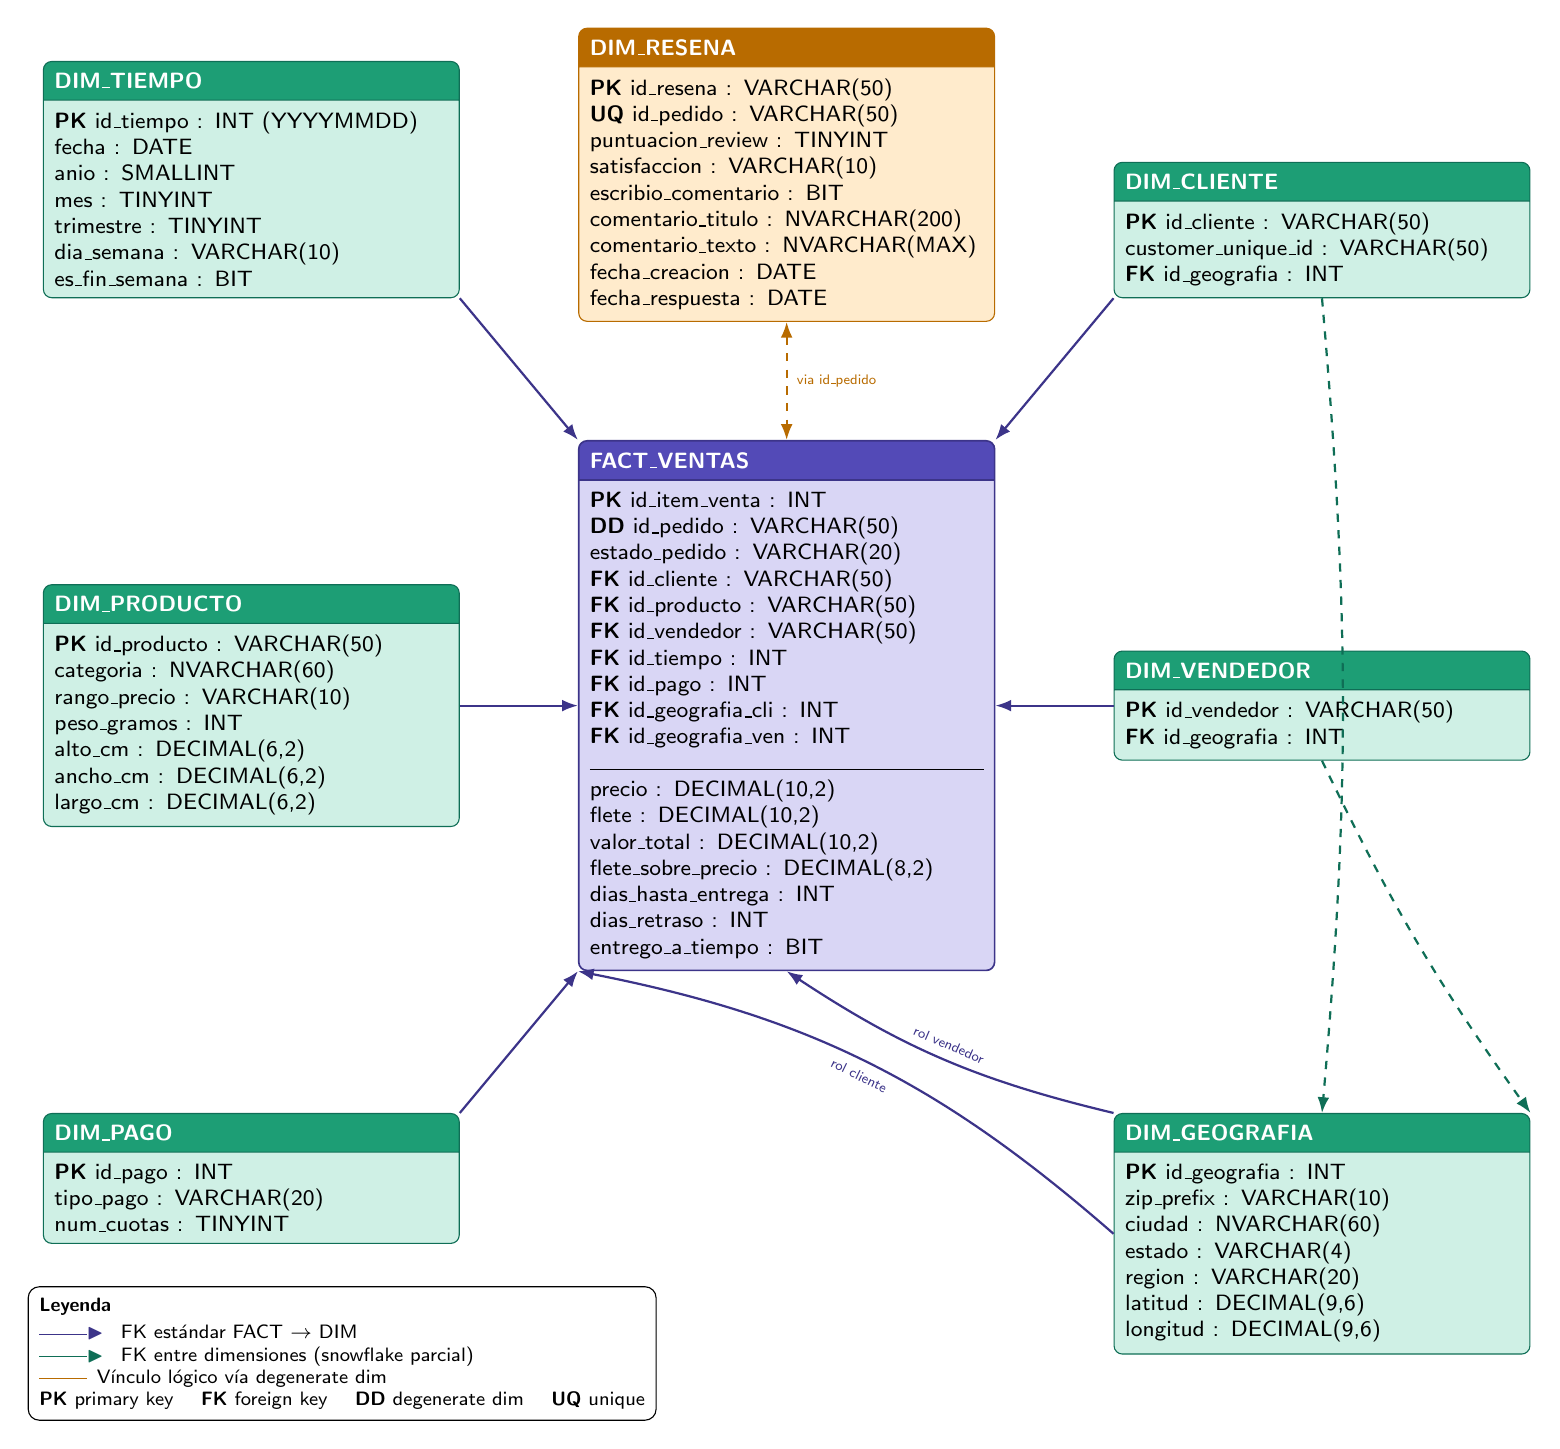
\begin{tikzpicture}[
    every node/.style={font=\footnotesize},
    tablestyle/.style={
        rectangle split,
        rectangle split parts=2,
        draw,
        line width=0.4pt,
        rounded corners=3pt,
        inner sep=4pt,
        text width=5.0cm,
        align=left,
    },
    fact/.style={
        tablestyle,
        rectangle split part fill={headerColor, factColor!30},
        draw=factBorder,
        line width=0.6pt,
    },
    dim/.style={
        tablestyle,
        rectangle split part fill={dimHeader, dimColor!50},
        draw=dimBorder,
    },
    resena/.style={
        tablestyle,
        rectangle split part fill={resenaHeader, resenaColor!50},
        draw=resenaBorder,
    },
    header/.style={
        text=white,
        font=\footnotesize\bfseries,
    },
    rel/.style={
        -{Latex[length=2mm, width=1.5mm]},
        thick,
        color=factBorder,
    },
    relgeo/.style={
        -{Latex[length=2mm, width=1.5mm]},
        thick,
        color=dimBorder,
        dashed,
    },
    relresena/.style={
        {Latex[length=2mm, width=1.5mm]}-{Latex[length=2mm, width=1.5mm]},
        thick,
        color=resenaBorder,
        dashed,
    },
]

% ===== FACT (centro) =====
\node[fact] (fact) at (0,0) {
    \nodepart{one}\textcolor{white}{\textbf{FACT\_VENTAS}}
    \nodepart{two}
    \textbf{PK} id\_item\_venta : INT\\
    \textbf{DD} id\_pedido : VARCHAR(50)\\
    estado\_pedido : VARCHAR(20)\\
    \textbf{FK} id\_cliente : VARCHAR(50)\\
    \textbf{FK} id\_producto : VARCHAR(50)\\
    \textbf{FK} id\_vendedor : VARCHAR(50)\\
    \textbf{FK} id\_tiempo : INT\\
    \textbf{FK} id\_pago : INT\\
    \textbf{FK} id\_geografia\_cli : INT\\
    \textbf{FK} id\_geografia\_ven : INT\\
    \hrulefill\\
    precio : DECIMAL(10,2)\\
    flete : DECIMAL(10,2)\\
    valor\_total : DECIMAL(10,2)\\
    flete\_sobre\_precio : DECIMAL(8,2)\\
    dias\_hasta\_entrega : INT\\
    dias\_retraso : INT\\
    entrego\_a\_tiempo : BIT
};

% ===== Fila superior =====
\node[dim, above left=1.8cm and 1.5cm of fact] (tiempo) {
    \nodepart{one}\textcolor{white}{\textbf{DIM\_TIEMPO}}
    \nodepart{two}
    \textbf{PK} id\_tiempo : INT (YYYYMMDD)\\
    fecha : DATE\\
    anio : SMALLINT\\
    mes : TINYINT\\
    trimestre : TINYINT\\
    dia\_semana : VARCHAR(10)\\
    es\_fin\_semana : BIT
};

\node[resena, above=1.5cm of fact] (resena) {
    \nodepart{one}\textcolor{white}{\textbf{DIM\_RESENA}}
    \nodepart{two}
    \textbf{PK} id\_resena : VARCHAR(50)\\
    \textbf{UQ} id\_pedido : VARCHAR(50)\\
    puntuacion\_review : TINYINT\\
    satisfaccion : VARCHAR(10)\\
    escribio\_comentario : BIT\\
    comentario\_titulo : NVARCHAR(200)\\
    comentario\_texto : NVARCHAR(MAX)\\
    fecha\_creacion : DATE\\
    fecha\_respuesta : DATE
};

\node[dim, above right=1.8cm and 1.5cm of fact] (cliente) {
    \nodepart{one}\textcolor{white}{\textbf{DIM\_CLIENTE}}
    \nodepart{two}
    \textbf{PK} id\_cliente : VARCHAR(50)\\
    customer\_unique\_id : VARCHAR(50)\\
    \textbf{FK} id\_geografia : INT
};

% ===== Laterales =====
\node[dim, left=1.5cm of fact] (producto) {
    \nodepart{one}\textcolor{white}{\textbf{DIM\_PRODUCTO}}
    \nodepart{two}
    \textbf{PK} id\_producto : VARCHAR(50)\\
    categoria : NVARCHAR(60)\\
    rango\_precio : VARCHAR(10)\\
    peso\_gramos : INT\\
    alto\_cm : DECIMAL(6,2)\\
    ancho\_cm : DECIMAL(6,2)\\
    largo\_cm : DECIMAL(6,2)
};

\node[dim, right=1.5cm of fact] (vendedor) {
    \nodepart{one}\textcolor{white}{\textbf{DIM\_VENDEDOR}}
    \nodepart{two}
    \textbf{PK} id\_vendedor : VARCHAR(50)\\
    \textbf{FK} id\_geografia : INT
};

% ===== Fila inferior =====
\node[dim, below left=1.8cm and 1.5cm of fact] (pago) {
    \nodepart{one}\textcolor{white}{\textbf{DIM\_PAGO}}
    \nodepart{two}
    \textbf{PK} id\_pago : INT\\
    tipo\_pago : VARCHAR(20)\\
    num\_cuotas : TINYINT
};

\node[dim, below right=1.8cm and 1.5cm of fact] (geografia) {
    \nodepart{one}\textcolor{white}{\textbf{DIM\_GEOGRAFIA}}
    \nodepart{two}
    \textbf{PK} id\_geografia : INT\\
    zip\_prefix : VARCHAR(10)\\
    ciudad : NVARCHAR(60)\\
    estado : VARCHAR(4)\\
    region : VARCHAR(20)\\
    latitud : DECIMAL(9,6)\\
    longitud : DECIMAL(9,6)
};

% ===== Relaciones FK estándar (FACT → DIMs) =====
\draw[rel] (tiempo.south east) -- (fact.north west);
\draw[rel] (cliente.south west) -- (fact.north east);
\draw[rel] (producto.east) -- (fact.west);
\draw[rel] (vendedor.west) -- (fact.east);
\draw[rel] (pago.north east) -- (fact.south west);

% ===== Relaciones role-playing DIM_GEOGRAFIA (2 roles) =====
\draw[rel] (geografia.north west) to[bend left=10]
    node[midway, sloped, above, font=\tiny] {rol vendedor} (fact.south);
\draw[rel] (geografia.west) to[bend right=15]
    node[midway, sloped, below, font=\tiny] {rol cliente} (fact.south west);

% ===== DIM_RESENA <-> FACT vía id_pedido (no FK formal, grano distinto) =====
\draw[relresena] (resena.south) -- node[midway, right, font=\tiny] {via id\_pedido} (fact.north);

% ===== FKs entre dimensiones (snowflake parcial) =====
\draw[relgeo] (cliente.south) to[bend left=5] (geografia.north);
\draw[relgeo] (vendedor.south) to[bend right=5] (geografia.north east);

% ===== Leyenda =====
\node[draw, rounded corners, fill=white, inner sep=4pt, below left=4cm and -1cm of fact, align=left, font=\scriptsize]
{
    \textbf{Leyenda} \\[2pt]
    {\color{factBorder}\rule[0.5ex]{0.6cm}{0.4pt}}{\color{factBorder}$\blacktriangleright$} \, FK estándar FACT $\rightarrow$ DIM \\
    {\color{dimBorder}\rule[0.5ex]{0.6cm}{0.4pt}}{\color{dimBorder}$\blacktriangleright$} \, FK entre dimensiones (snowflake parcial) \\
    {\color{resenaBorder}\rule[0.5ex]{0.6cm}{0.4pt}}\, Vínculo lógico vía degenerate dim \\
    \textbf{PK} primary key \quad \textbf{FK} foreign key \quad \textbf{DD} degenerate dim \quad \textbf{UQ} unique
};

\end{tikzpicture}

\end{document}
